%----------------------------------------------------------------------------------------
%	SECTION 3
%----------------------------------------------------------------------------------------
\section{Simulation Results (walking model)}\label{simulation}
In this section a method to analyze the stability of the system is displayed regarding the model in section (\ref{walkingmodel}). The fourth order Runge-Kutta method \cite{runge} was applied in order to simulate the Eqs. (\ref{eq.singlesuppx})-(\ref{eq.doublesuppy}). A different time steps were  used for different situations.
\subsection{Fixed points}\label{pontosfixos}
We are interested in determining the fixed points of the system, this is, the points which repeat after an iteration for a grid of associated parameters. This way, we determine the Poincaré section which we will define by, instead of $\psi_n=[y_n,\theta_n]$, as  $\psi_n=[y_n,\Delta x_n]$ \footnote{The definition of the Poincaré section is done this way because the difference in length of the stride provides a more accurate measurement on  the fixed points} and the subsequent Poincaré section $\psi_{n+1}=[y_{n+1},\Delta x_{n+1}]$. Some of the parameters were kept fixed such as the spring stiffness $k=14000$ N/m, the spring rest length $l_0=1$ m, the mass, $m=80$ Kg and the angle of the initial velocity at VLO $\beta=0$.

The grid in which the model was studied consists on the variation of 3 parameters, the energy $E$  which changes the initial velocity of the leg and has a variation in the interval $[800,840]$ J with $\Delta E = 1$J, the angle of attack $\alpha$ which changes the aperture of the leg and it was studied by dividing the interval $[\pi/2-\pi/5,\pi/2]$ rad into 30 subintervals to access each angle in this range. Also, the initial position $y_0$ was studied by dividing the interval $[l_0 \sin{\theta}, l_0]$ into 25 subintervals. This way the parameter space contains $40 \times 30 \times 25 = 30000$ possible configurations in which the system can be stable. Out of all of this possibilities a filtering was applied based on which configurations had successfully completed 2 strides with a time step on the Runge-Kutta of $\Delta t= 0.001$ s.

The criteria for failling to complete a simulation is the same as in the previous section (\ref{walkingmodel}),this is, configurations in which the center of mass falls ($y<0$) or goes backwards ($v_x<0$) or leaves the ground ($y>l_0$), were not suitable as valid candidates for stable configurations of the system. The results of this filtering were that 8195 out of 30000 configurations had successfully completed 2 strides and were selected as candidates for fixed points.

Having this subset of fixed point candidates, configurations in which the differences $|\Delta x_2-\Delta x_1|< 0.001$, $|(y_1-y_0)|<0.001$ and $(y_2-y_1)|<0.001$ were elligible as fixed points. After determining the fixed points, it is important to know if they are associated with a stable or unstable region. We can do this by determining the eigenvalues of the Jacobian \cite{Seyfarth2006},
\begin{equation}
 J= \begin{bmatrix}
    \frac{\partial \Delta x_{n+1}}{\partial \Delta x_{n}} & \frac{\partial \Delta x_{n+1}}{\partial  y_{n}}\\
     \frac{\partial  y_{n+1}}{\partial \Delta x_{n}} & \frac{\partial y_{n+1}}{\partial  y_{n}}
  \end{bmatrix},
  \label{eigeneq}
  \end{equation}
\noindent where each derivative can be computed by the following expression,
\begin{equation}
    \frac{\partial \Delta x_{n+1}}{\partial \Delta x_{n}}=  \frac{\frac{\partial \Delta x_{n+1}}{\partial t}}{\frac{\partial \Delta x_{n}}{\partial t}}. 
\end{equation}
If the eigenvalues of the fixed point lie in the circle of radius 1, this is, if $|\lambda_{1,2}|<1$, then the fixed point is considered stable, otherwise, is considered a unstable point \cite{Strogatz2001}. With this, in the subset of 8195 configurations which completed 2 strides, 11 were selected as fixed points, in Table (\ref{tabela}) the parameters for this points are displayed aswell as the respective eigenvalues of matrices (\ref{eigeneq}).

\begin{table}[H]
 \centering
\begin{tabular}{c|c|c|c|c|c}
Energy{[}J{]} &  $\alpha_0$ & $y_0${[}m{]} & $\lambda_1$ & $\lambda_2$ & Stability \\ \hline
800 & 1.215 & 0.950 & 0.629 & 0 & Stable \\
801 & 1.152 & 0.962 & 1.711 & 0 & Unstable \\
809 & 1.131 & 0.970 & 1.388 & 0 & Unstable \\
812 & 1.236 & 0.953 & 1.860 & 0 & Unstable \\
814 & 1.131 & 0.973 & 1.144 & 0 & Unstable \\
821 & 1.089 & 0.982 & 0.536 & 0 & Stable \\
825 & 1.110 & 0.983 & 1.044 & 0 & Unstable \\
827 & 1.236 & 0.947 & -1.063 & 0 & Unstable \\
828 & 1.089 & 0.986 & 0.734 & 0 & Stable \\
834 & 1.089 & 0.991 & 0.739 & 0 & Stable \\
839 & 1.068 & 0.995 & 0.467 & 0 & Stable
\end{tabular}
\caption{Fixed points table regarding the walking model. In this table we can see that if the energy is higher, the points with higher stability will be those with smaller angles, otherwise the case is reversed.}
\label{tabela}
\end{table}

\subsection{Step incrementation}
Having determined the fixed points and their respective type, an estimation of the stable and unstable zones of the parameter space was determined. This was done by incrementing the step of the configurations that completed 2 strides (\ref{pontosfixos}), so that the maximum number of steps,$maxsteps$, increases by 1 from [3,10] with a Runge-Kutta time step of $\Delta t=0.00075$ s. If the simulation registered a success when the step was incremented, we increment another step, otherwise, we associate to that configuration a maximum number of steps of $maxsteps-1$. If a configuration point reached 10 steps, we registered the number of steps to that configuration to be $maxsteps$.
Fig. (\ref{step_10}) shows the final result obtained aswell with the points that succeeded 10 steps as the fixed points associated.
\begin{figure}[H]
  \centering
  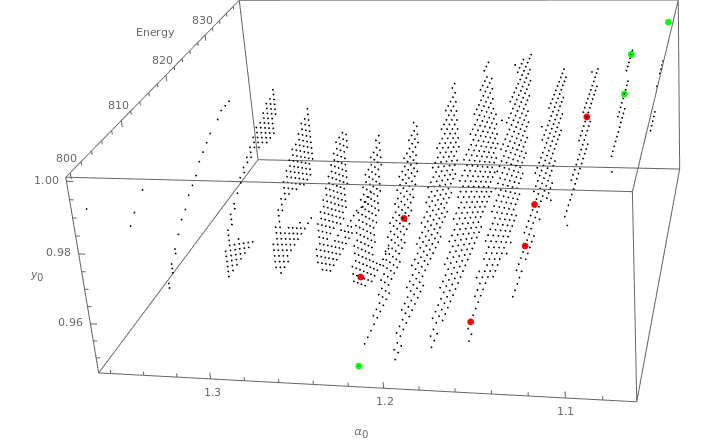
\includegraphics[width=0.7\textwidth]{Step10fixedpoints.png}
  \caption{Successful 10 step configurations with stable fixed points in green and unstable fixed points in red. In this 3D plot the Energy was varied from 800 and 840, $y_0$ from 0.8 to 1 and $\alpha_0$ from 0.94 to 1.57 and only this configurations remained. The fixed points displayed are associated to Table (\ref{tabela}). There is a preference for the stable configurations to have angle of attack of $\approx$ [1.05,1.25]}
  \label{step_10}
  \end{figure}

Figures (\ref{estavel}) and (\ref{unstable}) simulate the behaviour of the Center of Mass in the walking model for respectively a stable and an unstable fixed point a constant angle of attack policy.
\begin{figure}[H]
  \centering
  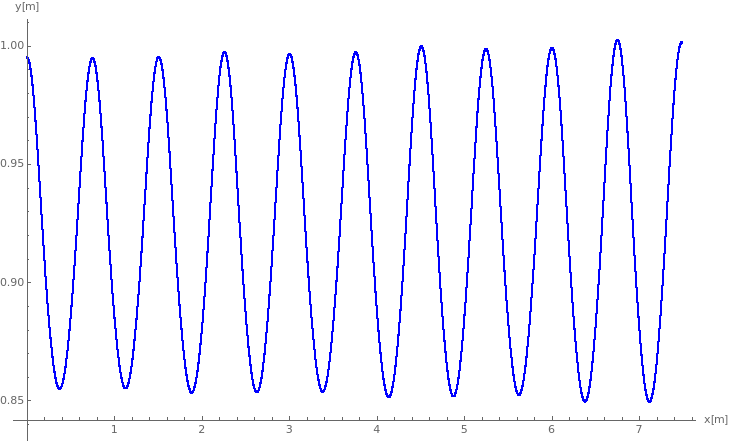
\includegraphics[width=0.65\textwidth]{Stable10steps.png}
  \caption{Position of the CoM of the stable fixed point E=839J, $\alpha_0$= 1.068,$y_0$=0.995, Runge-Kutta timestep $\Delta t=0.0005$s. In this example, the fixed point successfully covers all 10 strides with no instability. }
  \label{estavel}
\end{figure}


\begin{figure}[H]
  \centering
  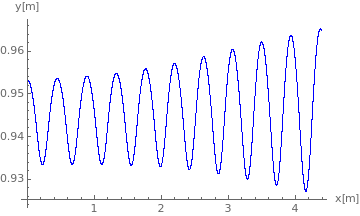
\includegraphics[width=0.65\textwidth]{unstableconfiguration.png}
  \caption{Position of the CoM of the unstable fixed point E=812J, $\alpha_0$= 1.236,$y_0$=0.953, Runge-Kutta timestep $\Delta t=0.0005$s. In this example, the fixed point successfully covers all 10 strides, but the amplitude increases in each stride bringing the system to an unstable configuration. }
  \label{unstable}
\end{figure}




